\documentclass[prd,amssymb,amsmath,amsfonts,nofootinbib,reprint,showpacs,longbibliography]{revtex4-1}

\usepackage{graphicx}
\usepackage{lmodern}
\usepackage{amsmath,amssymb}
\usepackage{mathrsfs}
\usepackage{amsfonts}
\usepackage[utf8]{inputenc}
\usepackage{url}
\usepackage[colorlinks]{hyperref}
\usepackage[table]{xcolor}
\usepackage{multirow}
\usepackage[normalem]{ulem}
\usepackage{lipsum}

\usepackage{marvosym}
\usepackage{enumerate}
\usepackage{color,soul}
\usepackage{acronym}

\usepackage{bm}
\usepackage{color}
\usepackage{commath}
\allowdisplaybreaks
\usepackage{multirow}

\def\lm{{\ell m}}
\newcommand{\avg}[1]{\rangle{#1}\langle}
\newcommand{\scri}{{\mathrsfs{I}}}
\newcommand{\stf}[1]{{\langle {#1} \rangle}}
\newcommand{\ord}{\mathcal{O}}
\newcommand{\f}{\frac}
\newcommand{\gsf}{\text{1GSF}}
\newcommand{\bk}{\text{0GSF}}
\newcommand{\el}{\ell}
\newcommand{\nn}{\nonumber}
\newcommand{\mbf}[1]{\mathbf{#1}}
\newcommand{\LOhat}{\!\hat{\,\mathbf{L}}_0}
\newcommand{\Lhat}{\!\hat{\,\mathbf{L}}_\text{N}}
\newcommand{\Jhat}{\hat{\mathbf{J}}_\text{N}}
\newcommand{\Sa}{\mbf{S}_1}
\newcommand{\Sb}{\mbf{S}_2}
\newcommand{\hs}{\hat{s}}
\newcommand{\hS}{\hat{S}}
\newcommand{\Lhatdot}{\dot{\hat{\,\mathbf{L}}}_\text{N}}
\newcommand{\LhatdotNew}{\dot{\hat{\,\mathbf{L}}}_{\text{N},\perp}}
\newcommand{\Sadot}{\dot{\mbf{S}}_1}
\newcommand{\Sbdot}{\dot{\mbf{S}}_2}
\newcommand{\Jdot}{\dot{\mbf{J}}}
\newcommand{\rdot}{\dot{\mbf{r}}}
\newcommand{\vdot}{\dot{\mbf{v}}}
\newcommand{\ud}{\mathrm{d}}
\newcommand{\Ldot}{\dot{\mbf{L}}_{\text N}}
\newcommand{\LN}{\mbf{L}_{\text N}}
\newcommand{\nnm}{\nonumber}
\newcommand{\mce}{\mathcal{E}}
\newcommand{\mcb}{\mathcal{B}}

\def\TEOBResumS{\texttt{TEOBResumS}}
\def\TEOBResumSGIOTTO{\texttt{TEOBResumSGIOTTO}}
\def\TEOBResumSecce{\texttt{TEOBResumSecce}}
\def\bajes{\texttt{bajes}}
\def\Boldtheta{\boldsymbol{\theta}}
\def\Boldd{\textbf{d}}
\def\TEOBResumSDali{\texttt{TEOBResumS-Dalí}}
\def\TEOBB{\texttt{Beyond-TEOBResumS}}
\def\c3{c_{\rm{N}^3\rm{LO}}}
\def\mbhf{M_{\rm BH}^f}
\def\abhf{a_{\rm BH}^f}
\def\alphalm0{\alpha_{\ell m 0}}
\def\taulm0{\tau_{\ell m 0}}
\def\omegalm0{\omega_{\ell m 0}}


% Define capitalized acronyms
\newacro{adm}[ADM]{Arnowitt-Deser-Misner}
\newacro{bbh}[BBH]{binary black hole}
% \newacroplural{bbh}[BBHs]{binary black holes}
\newacro{bh}[BH]{black hole}
\newacroplural{bh}[BHs]{black holes}
\newacro{bhns}[BHNS]{black hole-neutron star}
\newacro{bhpt}[BHPT]{black hole perturbation theory}
\newacro{bns}[BNS]{binary neutron star}
\newacro{bf}[BF]{Bayes' factor}
\newacro{cbc}[CBC]{compact binary coalescence}
\newacro{ce}[CE]{Cosmic Explorer}
\newacro{da}[DA]{data analysis}
\newacro{et}[ET]{Einstein Telescope}
\newacro{eob}[EOB]{Effective-One-Body}
\newacro{eom}[EOM]{equations of motion}
\newacro{fd}[FD]{frequency domain}
\newacro{fft}[FFT]{Fast Fourier transform}
\newacro{gw}[GW]{gravitational-wave}
\newacroplural{gw}[GWs]{Gravitational-waves}
\newacro{gr}[GR]{general relativity}
\newacro{grb}[GRB]{gamma-ray burst}
\newacro{grhd}[GRHD]{general-relativistic hydrodynamics}
\newacro{gwosc}[GWOSC]{Gravitational Wave Open Science Center}
\newacro{gwtc1}[GWTC-1]{the first gravitational-wave transients catalog}
\newacro{gsf}[GSF]{Gravitational Self Force}
\newacro{hm}[HM]{Higher mode}
\newacroplural{hm}[HMs]{Higher modes}
\newacro{ifo}[IFO]{interferometer}
\newacro{imr}[IMR]{inspiral-merger-ringdown}
\newacro{im}[IMR]{inspiral-to-merger}
\newacro{kagra}[KAGRA]{Kamioka Gravitational Wave Detector}
\newacro{ligo}[LIGO]{Laser Interferometer Gravitational-Wave Observatory}
\newacro{lisa}[LISA]{Laser Interferometer Space Antenna}
\newacro{lr}[LR]{Light Ring}
\newacro{lso}[LSO]{Last Stable Orbit}
\newacro{lvc}[LVC]{LIGO-Virgo Collaboration}
\newacro{lvk}[LVK]{LIGO-Virgo-Kagra Collaboration}
\newacro{lo}[LO]{leading order}
\newacro{ns}[NS]{neutron star}
\newacroplural{ns}[NSs]{neutron stars}
\newacro{nr}[NR]{numerical relativity}
\newacro{nqc}[NQC]{Next-to-quasicircular corrections}
\newacro{nlo}[NLO]{next-to-leading order}
\newacro{nnlo}[NNLO]{next-to-next-to-leading order}
\newacro{n3lo}[N3LO]{next-to-next-to-next-to-leading order}
\newacro{n4lo}[N3LO]{next-to-next-to-next-to-next-to-leading order}
\newacro{ode}[ODE]{Ordinary Differential Equation}
\newacroplural{ode}[ODEs]{Ordinary Differential Equations}
\newacro{pn}[PN]{post-Newtonian}
\newacro{pm}[PM]{post-Minkowskian}
\newacro{pe}[PE]{parameter estimation}
\newacro{psd}[PSD]{power spectral density}
\newacro{pa}[PA]{post-adiabatic}
\newacro{qnm}[QNM]{quasi-normal mode}
\newacro{qc}[QC]{quasi-circular}
\newacro{snr}[SNR]{signal-to-noise ratio}
\newacro{spa}[SPA]{stationary-phase approximation}
\newacro{sxs}[SXS]{Simulating eXtreme Spacetimes}
\newacro{td}[TD]{time domain}
\newacro{ng}[NG]{Nect Generation}


\definecolor{cyan}{rgb}{0,0.9,0.9}
\definecolor{orange}{rgb}{0.9,0.5,0}
\definecolor{magenta}{rgb}{1,0,1}
\definecolor{purple}{rgb}{0.8,0.4,0.8}
\definecolor{gray}{rgb}{0.8242,0.8242,0.8242}
\definecolor{dodgerblue}{rgb}{0.12, 0.56, 1.0}

\newcommand{\RG}[1]{{\textcolor{dodgerblue}{{RG: #1}} }}
\newcommand{\JL}[1]{{\textcolor{purple}{{JL: #1}} }}
\newcommand{\DC}[1]{{\textcolor{orange}{{DC: #1}} }}
\newcommand{\NC}[1]{{\textcolor{magenta}{{NC: #1}} }}


\newcommand{\todo}[1]{\textcolor{red}{\texttt{TODO: #1}}} 
\newcommand{\red}[1]{\textcolor{red}{#1}} 
\newcommand{\bl}[1]{\textcolor{blue}{#1}} 
\newcommand{\cor}[2]{\sout{#1}\textcolor{red}{#2}} 
\newcommand{\old}[1]{\textcolor{gray}{\sout{#1}}}
\newcommand{\new}[1]{\red{#1}}

\newcommand{\eo}[0]{\hat{E}_0}
\newcommand{\lo}[0]{\hat{L}_0}
\newcommand{\bphi}[0]{\bar{\varphi}}
\newcommand{\dbphi}[0]{\dot{\bar{\varphi}}}
\newcommand{\dphi}[0]{\dot{\varphi}}
\newcommand{\amrg}[1]{{A_{#1}^{\rm mrg}}}
\newcommand{\anqc}[1]{{A_{#1}^{\rm NQC}}}
\newcommand{\omgmrg}[1]{{\omega_{#1}^{\rm mrg}}}

\interfootnotelinepenalty=10000

\begin{document}

\title{Beyond-TEOBResumS}

\author{Nicol\'o \surname{Cibrario}${}^{1,2}$}
\author{Danilo \surname{Chiaramello}${}^{1,2}$}
\author{Jacob \surname{Lange}${}^{2}$}
%% \author{Rossella \surname{Gamba}${}^{3,4}$}

\affiliation{${}^{1}$Dipartimento di Fisica, Universit\`a di Torino, Via P. Giuria 1, 10125 Torino, Italy}
\affiliation{${}^{2}$ INFN Sezione di Torino, Torino, 10125, Italy}
%% \affiliation{${}^{3}$ Institute for Gravitation \& the Cosmos, The Pennsylvania State University, University Park PA 16802, USA}
%% \affiliation{${}^{4}$ Department of Physics, University of California, Berkeley, CA 94720, USA}

\begin{abstract}
\todo{Nicol\'o, Danilo, Jacob}
\Acp{gw} from \acp{bbh} allow us to test \ac{gr} in the strong-field, large curvature regime.
We present \TEOBB, a new parameterized \ac{bbh} model for null tests of \ac{gr}.
\TEOBB is based on the \TEOBResumSDali model, which incorporates non-circular orbits and spin precession.
We apply the model to both real and simulated \ac{gw} data, and show that \dots
\end{abstract}

\date{\today}
\maketitle

% reset all acronyms
\acresetall

\section{Introduction}
\todo{all}

\section{\TEOBB}
\todo{Danilo}

We build upon the most recent version of the generic \ac{bbh} model \TEOBResumSDali, incorporating non-circular
orbits and spin precession~\cite{Nagar:2024oyk, Gamba:2024cvy, Albanesi:2025txj}. The parametrized model is constructed by
allowing user-input deviations from a few of the \ac{nr}-informed quantities that enter the dynamics or waveform
template. Specifically, regarding the dynamical sector and the inspiral, we consider deviations from two
\ac{nr}-calibrated parameters: $a_6^c$, an effective 6\ac{pn} coefficient entering the (resummed) gravitational
potential $A(r)$, and $c_{\rm{N}^3\rm{LO}}$, a next-to-next-to-next-to-leading-order term in the spin-orbit
part of the Hamiltonian. We use in this case additive deviations from the fitted values:
\begin{subequations}
\begin{align}
a_6^c &\rightarrow a_6^c + \delta a_6^c \\
\c3 &\rightarrow \c3 + \delta \c3 \, .
\end{align}
\end{subequations}
Concerning the waveform model, the deformations we allow are the following:
\begin{itemize}
    \item A shift in the otherwise fixed value of $\Delta t_{\rm NQC}$, a parameter that determines the location
    of the peak amplitude of the model waveform and that of the \ac{nqc} extraction point with respect to the
    time when the pure orbital frequency $\Omega_{\rm orb}$ reaches a final peak. This parameter is set
    to $\Delta t_{\rm NQC} = 1M$ in the model, roughly extrapolating from the test-mass result. The implemented
    deviation is additive:
    \begin{equation}
    \Delta t_{\rm NQC} \rightarrow \Delta t_{\rm NQC} + \delta \Delta t_{\rm NQC}
    \end{equation}
    \item Fractional deviations from the mass and spin of the final remnant \ac{bh}, which determine the properties
    of the post-merger signal:
    \begin{subequations}
    \begin{align}
    \mbhf &\rightarrow \mbhf (1 + \delta \mbhf) \\
    \abhf &\rightarrow \abhf (1 + \delta \abhf)
    \end{align}
    \end{subequations}
    The bare values used in the standard version of the model are highly accurate fits of \ac{nr} data~\cite{paper}.
%
\item Deviations from the \ac{nr}-fitted values of the fundamental QNM frequencies (\DC{probably shouldn't call these frequencies})
$\sigma_{\ell m 0} = \alphalm0 + i \omegalm0$ of each mode. We separately allow fractional deformations of the oscillatory
term, $\omegalm0$, and either the damping time $\taulm0$ or inverse damping time $\alphalm0 = \taulm0^{-1}$:
\begin{subequations}
\begin{align}
\alphalm0 &\rightarrow \alphalm0 (1 + \delta \alphalm0) \\
\taulm0   &\rightarrow \taulm0   (1 + \delta \taulm0) \\
\omegalm0 &\rightarrow \omegalm0 (1 + \delta \omegalm0)
\end{align}
\end{subequations}
We require that the (inverse) damping time deviations satisfy $\delta \taulm0 > -1\  (\delta \alphalm0 > -1)$, to avoid exponentially growing
post-merger signals.
%
\item For each mode, we consider deviations from \ac{nr}-fitted values of the amplitude and frequency of the
waveform at merger, defined as the peak of the (co-precessing) $(2,2)$ mode. If a waveform mode is decomposed
as $h_{\ell m} = A_{\ell m} e^{-i \phi_{\ell m}}$ and $\omega_{\ell m} = d\phi_{\ell m}/dt$,
\begin{subequations}
\begin{align}
A_{\ell m}^{\rm mrg} &\rightarrow A_{\ell m}^{\rm mrg} (1 + \delta A_{\ell m}^{\rm mrg}) \\
\omega_{\ell m}^{\rm mrg} &\rightarrow \omega_{\ell m}^{\rm mrg} (1 + \delta \omega_{\ell m}^{\rm mrg})
\end{align}
\end{subequations}
%
\item For each mode, we also separately implement deviations from waveform properties measured at the \ac{nqc}
extraction point, $t_{\ell m}^{\rm NQC}$. We again use fractional deviations, so that:
\begin{subequations}
\begin{align}
x_{\ell m}^{\rm NQC} &\rightarrow x_{\ell m}^{\rm NQC} (1 + \delta x_{\ell m}^{\rm NQC}) \\
x &\in \{A, \dot{A}, \omega, \dot{\omega}\} \, .
\end{align}
\end{subequations}
\end{itemize}
%
A note on the NQC point deviations: currently the location of the \ac{nqc} point in \TEOBResumSDali~differs between modes. 
We have three different implementations:
\begin{itemize}

\item[(i)] For the $(2,2), (3,2), (4,2)$ and $(4,3)$ modes, the \ac{nqc} point is tied to the peak time of the $(2,2)$
mode amplitude of the EOB waveform, $t_{\ell m}^{\rm NQC} = t_{A_{22}^{\rm peak}}^{EOB} + 2 + \Delta t_{\ell m}$, 
where $t_{A_{22}^{\rm peak}}^{EOB} = t_{\Omega_{\rm orb}^{\rm peak}} - 2 - \Delta t_{\rm NQC}$, $t_{\Omega_{\rm orb}^{\rm peak}}$
is the time when the \textit{pure} orbital frequency peaks, $\Delta t_{\rm NQC} = 1$, and $\Delta t_{\ell m}$ is an \ac{nr}-fitted parameter
encoding the delay between the peak of a generic mode $(\ell, m)$ with respect to the $(2,2)$ mode.
The NQC extraction point thus falls in the post-merger part of the waveform, where the ringdown
template is valid; so, the amplitude, frequency and their derivatives can be computed by evaluating the
template at the appropriate time. This means that \textit{the merger time deviations also influence the NQC time
quantities}. This is desireable, as it means that the \ac{nqc} corrections will enforce a smooth connection between
the late inspiral and the ringdown.
\item[(ii)] For the $(5,5)$ mode, the \ac{nqc} point is located as defined above, but the \ac{nqc} quantities
are computed through direct \ac{nr} fits; in this case, the merger and NQC time deviations are completely independent.
\item[(iii)] For the $(2,1), (3,3)$ and $(4,4)$ modes, the NQC point coincides
with the peak of the $(2,2)$ mode, $t_{\ell m}^{\rm NQC} = t_{A_{22}^{\rm peak}}^{\rm EOB}$; direct \ac{nr} fits 
are used in these cases as well. Here, the merger and NQC amplitude and frequency deviations actually affect
the same physical quantities, while acting independently and entering the model at (slightly) different stages.
\end{itemize}

\subsection{Visualizing the effect of the deviations}

\begin{figure*}
    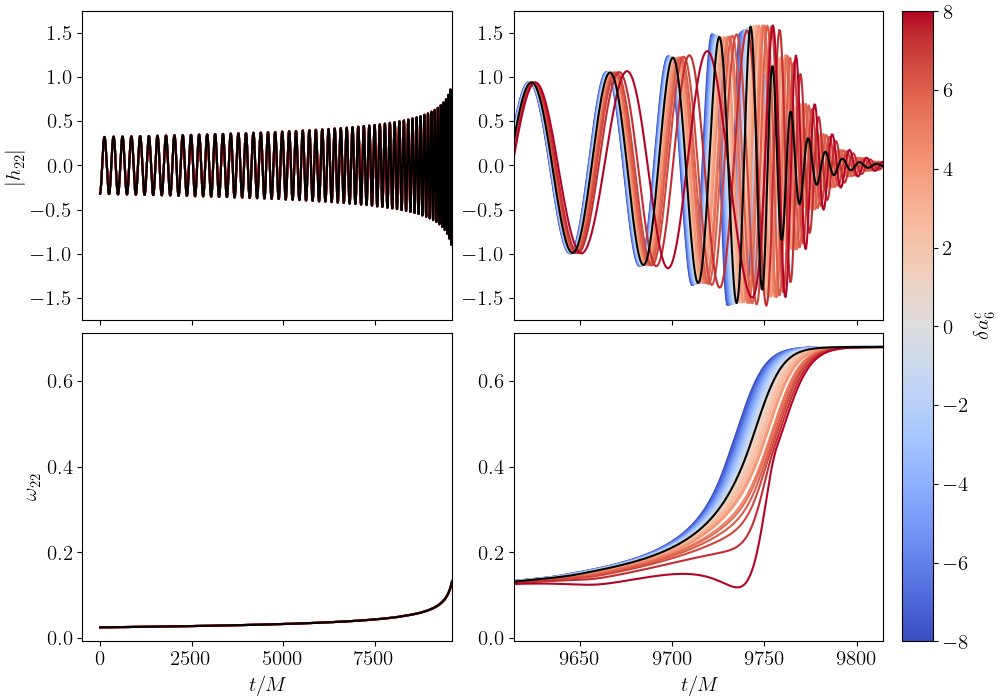
\includegraphics[width=0.49\textwidth]{figs/delta_a6c_-8.0_8.0.png}
    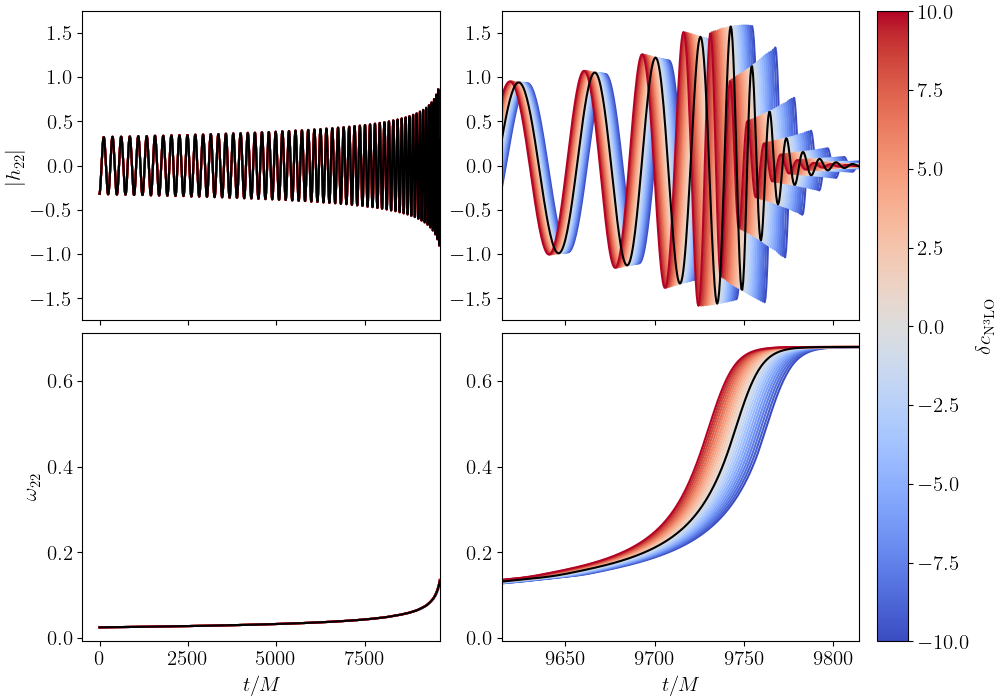
\includegraphics[width=0.49\textwidth]{figs/delta_cN3LO_-10.0_10.0.png}
    \caption{\label{fig:a6c3}
    Effect of the variation of $a_6^{\rm c}$ and $\c3$ on the $(2,2)$ mode real part and frequency
    for a binary with $q = 1, \chi_1 = \chi_2 = 0.6$. Waveforms here are aligned so they always start at $t = 0$,
    to better appreciate the cumulative effect of the deformed dynamics. $\delta a_6^c$ and $\delta \c3$ cause a slightly
    delayed or accelerated late inspiral and plunge, shifting the phase of the signal. The model is quite
    sensitive to the increase of $a_6^c$, delivering unphysical results for deviations $\geq 8$ in this case.
    This is partly due to the failure of the \ac{nqc} corrections in enforcing a smooth transition to the ringdown
    portion of the waveform. Dynamically, a broader range of values is allowed for $\delta a_{6}^c$, but
    if the deviation is large enough the warped potential leads to unphysical late dynamics.
    We see that an increase in $a_6^c$ delays the merger, while a decrease moves it forward slightly. The
    opposite is true for $\c3$ in this case; with negative spins it would instead be the same (i.e.,
    an increase in $\c3$ would delay the merger in that case).}
\end{figure*}

\begin{figure*}
    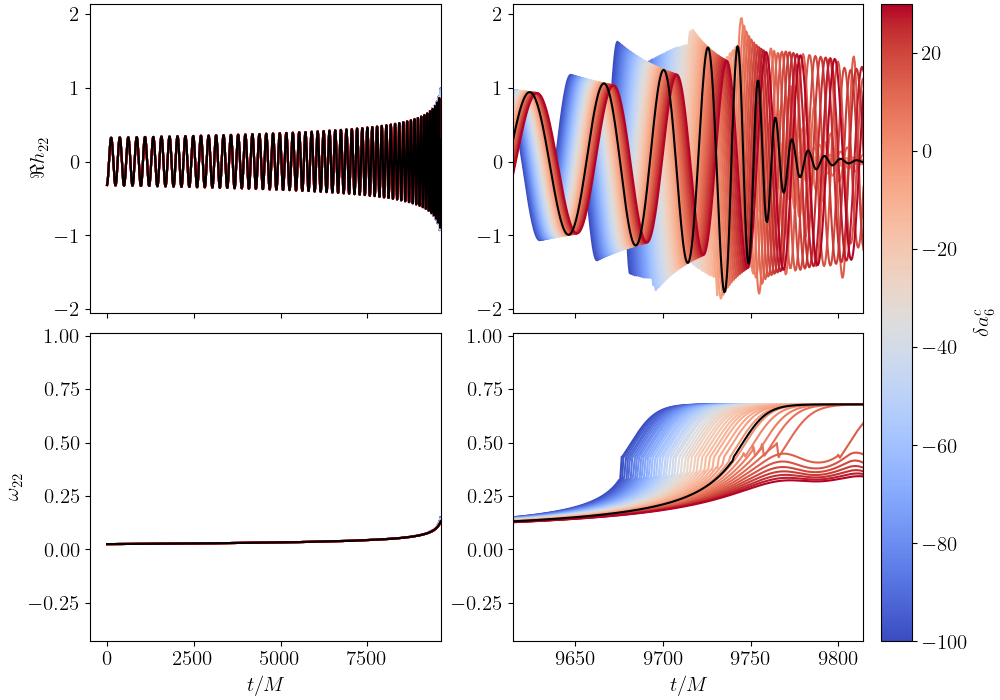
\includegraphics[width=0.49\textwidth]{figs/delta_a6c_-100.0_30.0.png}
    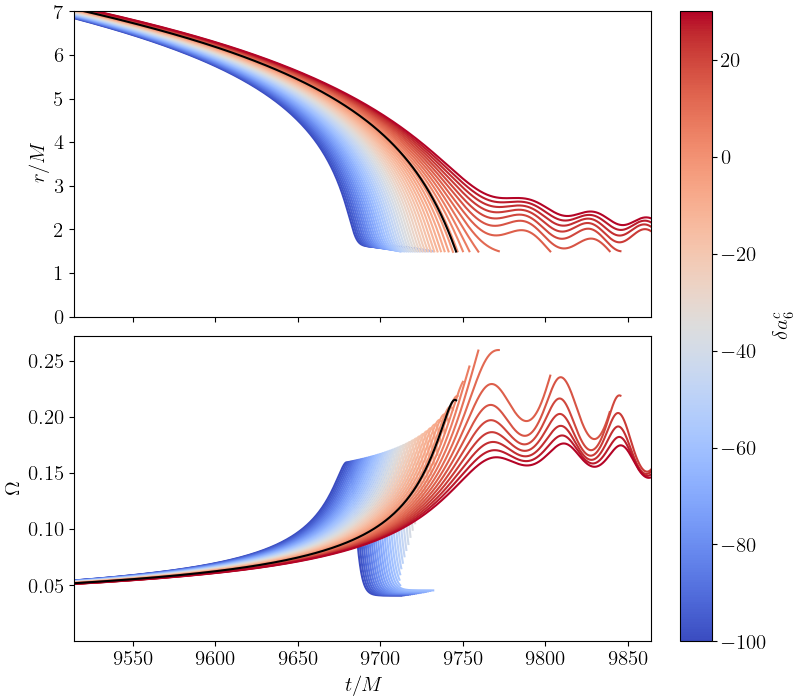
\includegraphics[width=0.49\textwidth]{figs/delta_a6c_-100.0_30.0_dyn.png}
    \caption{Effect of the variation of $a_6^{\rm c}$ on the $(2,2)$ mode real part and frequency (left) and the
    orbital dynamics (right), for a binary with $q = 1, \chi_1 = \chi_2 = 0.6$. \ac{nqc} corrections are not
    applied here.
    Waveforms here are aligned so they always start at $t = 0$, to better appreciate the cumulative effect of the
    deformed dynamics. Compared to Fig.~\ref{fig:a6c3}, $a_6^c$ here takes values in a much larger interval,
    only leading to pathological results when the misshaped potential $A$ leads to unphysical late dynamics.}
\end{figure*}

\begin{figure*}
    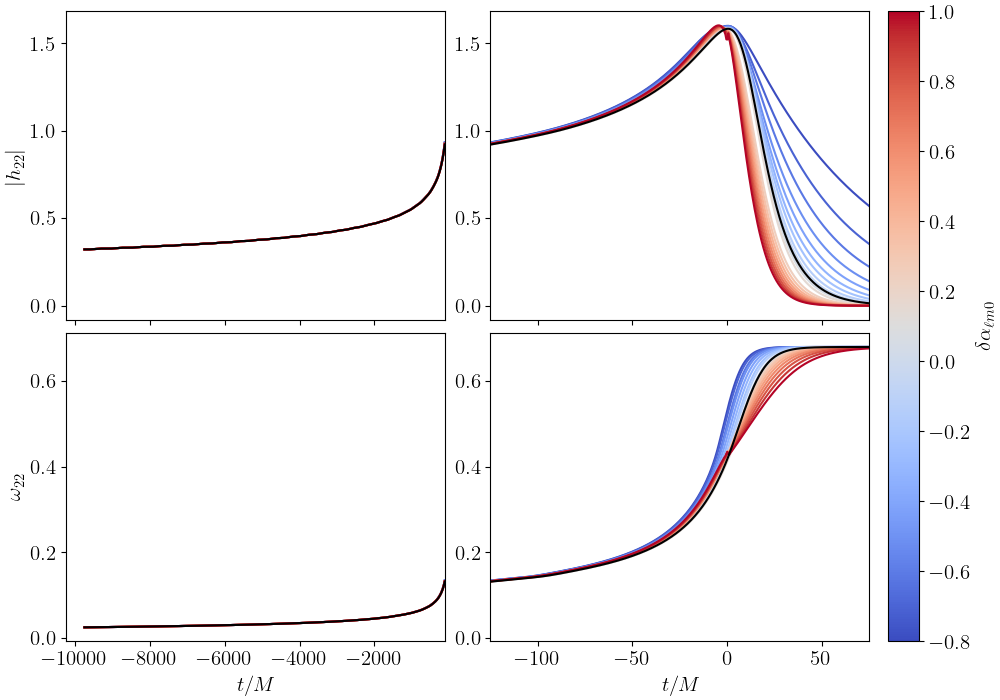
\includegraphics[width=0.49\textwidth]{figs/delta_alpha220_-0.8_1.0.png}
    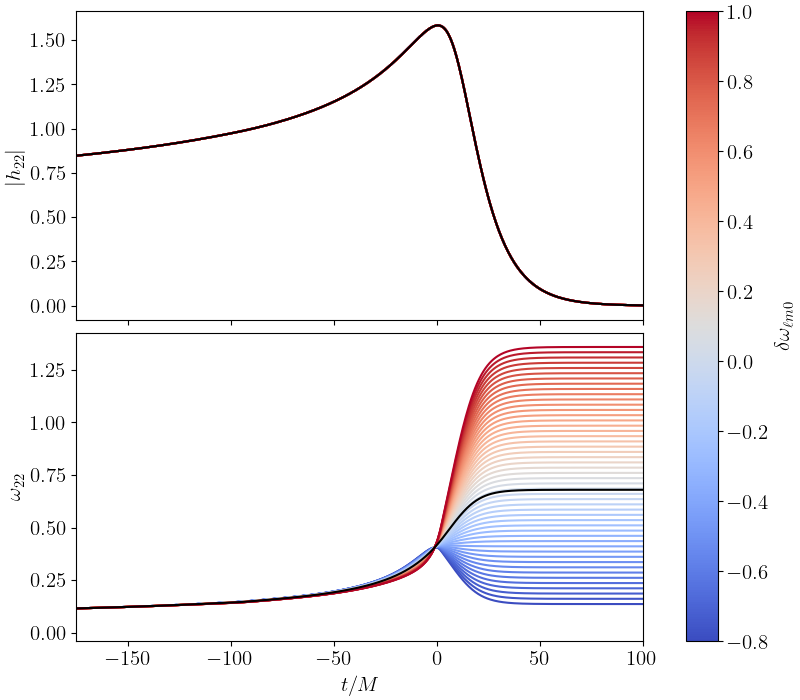
\includegraphics[width=0.49\textwidth]{figs/delta_omg220_-0.8_1.0.png}
    \caption{Effect of the variation of $\alpha_{220}$ and $\omega_{220}$ on the $(2,2)$ mode amplitude and frequency
    for a binary with $q = 1, \chi_1 = \chi_2 = 0.6$. Waveforms here are aligned so that for each
    $t = 0$ corresponds to the peak of $|h_{22}|$. An increase in the inverse damping time leads to a faster
    decaying ringdown, and vice-versa; this also affects the frequency evolution due to the structure of the
    ringdown model. Shifting the frequency does not instead significantly affect the amplitude.}
\end{figure*}

\begin{figure*}
    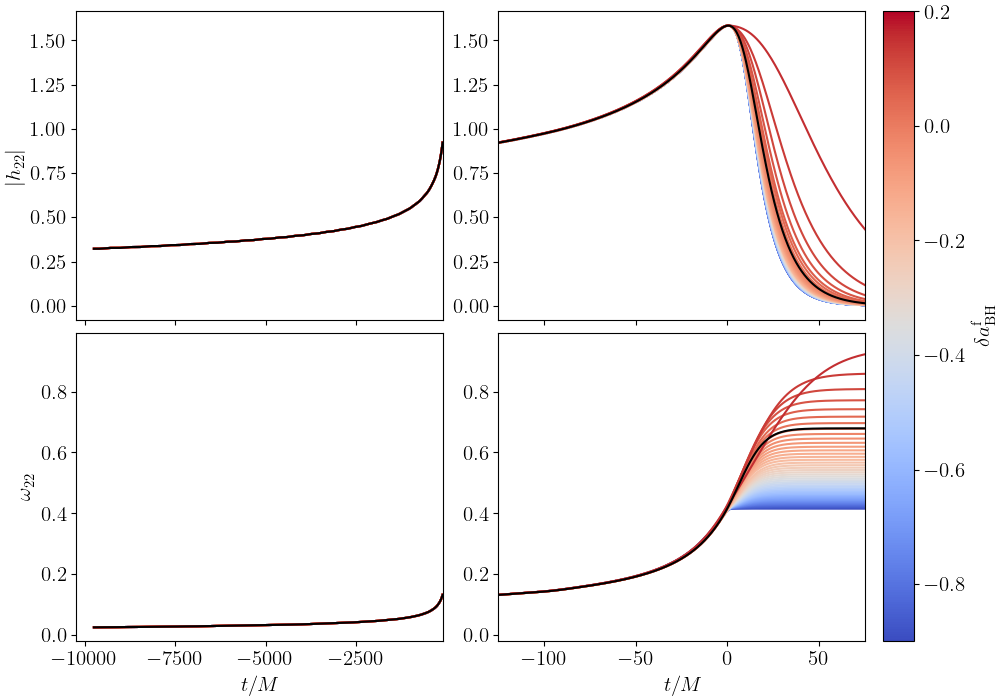
\includegraphics[width=0.49\textwidth]{figs/delta_abhf_-0.9_0.2.png}
    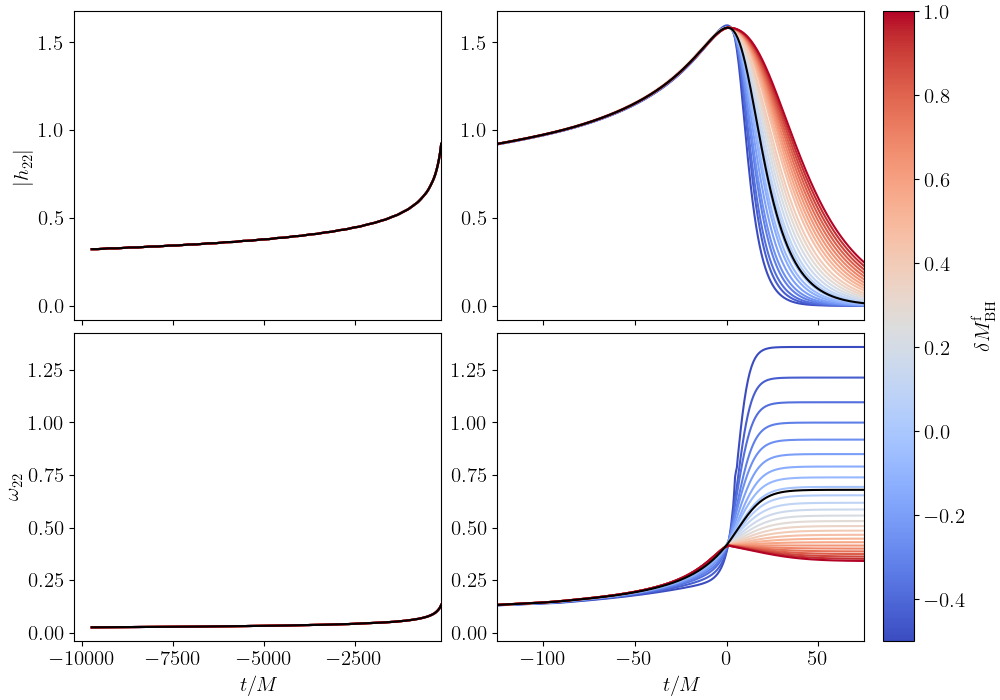
\includegraphics[width=0.49\textwidth]{figs/delta_Mbhf_-0.5_1.0.png}
    \caption{Effect of the variation of $\mbhf$ and $\abhf$ on the $(2,2)$ mode amplitude and frequency
    for a binary with $q = 1, \chi_1 = \chi_2 = 0.6$. Waveforms here are aligned so that for each
    $t = 0$ corresponds to the peak of $|h_{22}|$. An increase in the inverse damping time leads to a faster
    decaying ringdown, and vice-versa, as expected; this also affects the frequency evolution due to the structure of the
    ringdown model. Shifting the frequency does not instead significantly affect the amplitude.}
\end{figure*}

\begin{figure*}
    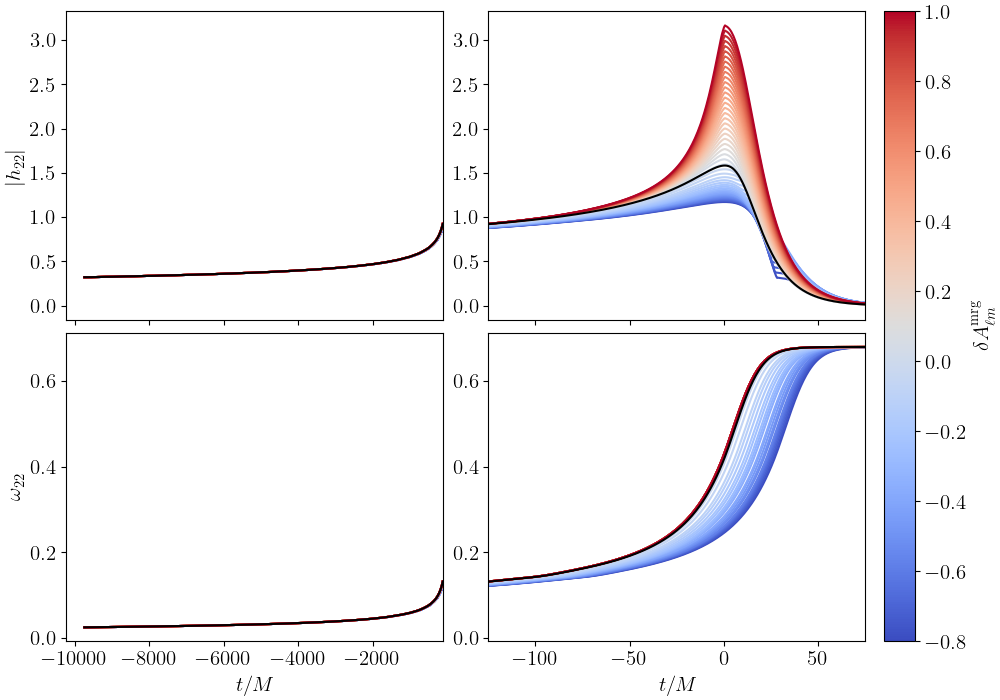
\includegraphics[width=0.49\textwidth]{figs/delta_A22_mrg_-0.8_1.0.png}
    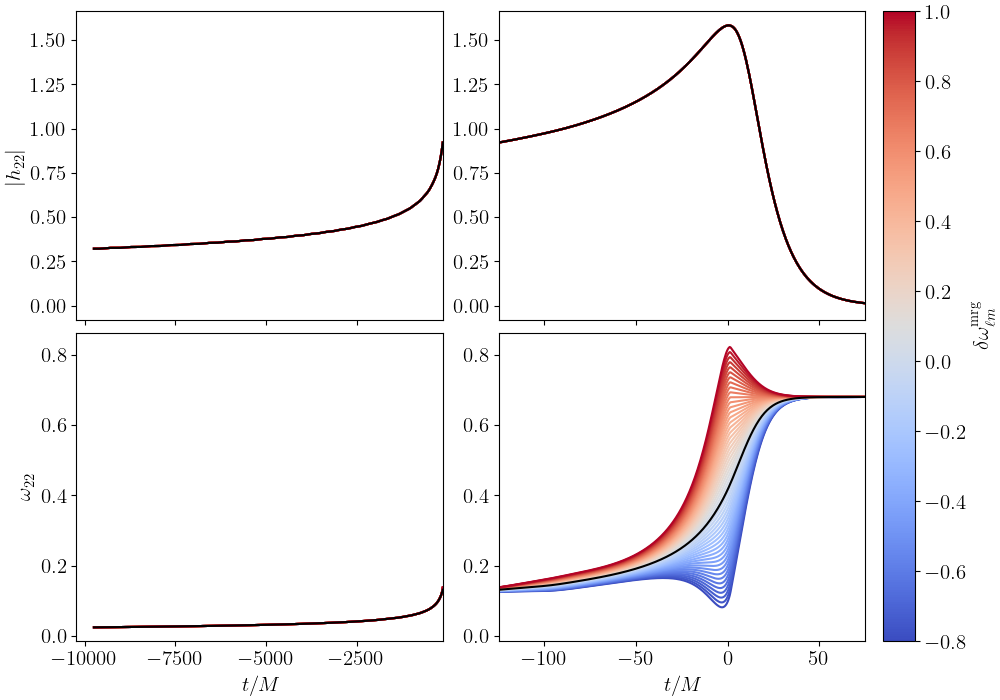
\includegraphics[width=0.49\textwidth]{figs/delta_Omg22_mrg_-0.8_1.0.png}
    \caption{Effect of the variation of $\amrg{22}$ and $\omgmrg{22}$ on the $(2,2)$ mode amplitude and frequency
    for a binary with $q = 1, \chi_1 = \chi_2 = 0.6$. Waveforms here are aligned so that for each
    $t = 0$ corresponds to the peak of $|h_{22}|$. Here we see how the shift in the merger quantities carries
    over to the NQC corrections, which enforce a match between the inspiral and ringdown. Increasing the amplitude
    does not change the location of the peak. Decreasing it however does (as is clear by the frequency plot),
    while also causing in the more extreme cases a non-smooth transition to the ringdown part of the signal.}
\end{figure*}

\begin{figure*}
    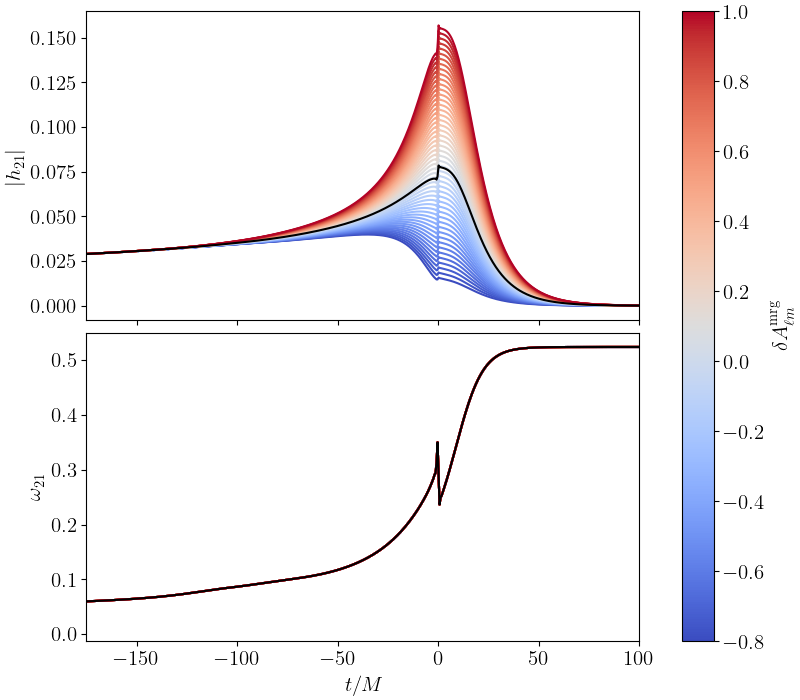
\includegraphics[width=0.49\textwidth]{figs/delta_A21_mrg_-0.8_1.0.png}
    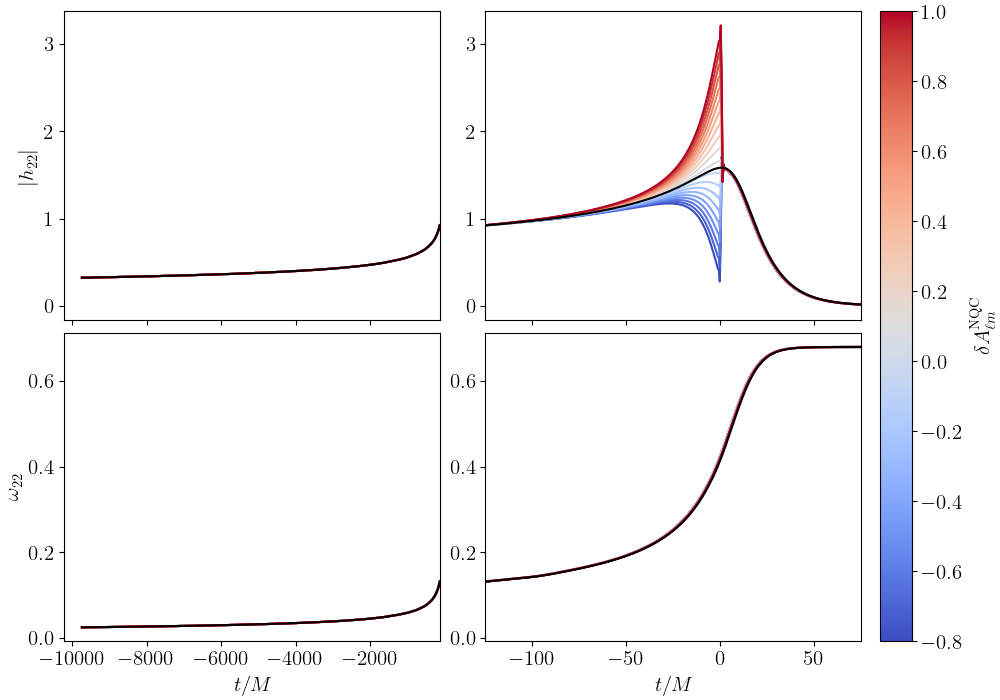
\includegraphics[width=0.49\textwidth]{figs/delta_A22_nqc_-0.8_1.0.png}
    \caption{\textit{Left:} Effect of the variation of $\amrg{21}$ on the $(2,1)$ mode of the waveform
    for a binary with $q = 2, \chi_1 = \chi_2 = 0.6$.
    For this multipole, the NQC point quantities are computed from a dedicated fit, with no direct link
    with the post-merger model, so the inspiral part does not link up smoothly with the ringdown.
    \textit{Right:} Variation of $\anqc{22}$ for a binary with $q = 1, \chi_1 = \chi_2 = 0.6$. The
    deformed NQC corrections here are not matched to a similarly modified post-merger signal, causing a discontinuity.}
\end{figure*}

\section{Application to data analysis}
\todo{Anyone who ran stuff, so Nic and Jake? }

\subsection{\ac{gw} \ac{pe}}
\todo{Quick recap of bayesian inference for GW}
\todo{Discuss settings for the \ac{pe} runs, e.g. sampler, priors, etc.}

\subsection{Model injections}
\RG{We may keep or nuke this section, depending on whether we want to. It is not strictly necessary,
but it does show that the model is same (and we could potentially discuss degeneracies among the deviation parameters,
e.g. final mass and spin vs damping time etc)}

\subsection{\ac{nr} injections}

\subsection{Real data}

\section{Conclusion}
\todo{all}

\bibliography{refs, local}

\end{document}
